\RequirePackage[l2tabu,orthodox]{nag}

% TODO: decide if one-sided/two-sided
%\documentclass[headsepline,footsepline,footinclude=false,fontsize=11pt,paper=a4,listof=totoc,bibliography=totoc,BCOR=12mm,DIV=12]{scrbook} % two-sided
\documentclass[headsepline,footsepline,footinclude=false,oneside,fontsize=11pt,paper=a4,listof=totoc,bibliography=totoc]{scrbook} % one-sided

\PassOptionsToPackage{table,svgnames,dvipsnames}{xcolor}

\usepackage[utf8]{inputenc}
\usepackage[T1]{fontenc}
\usepackage[sc]{mathpazo}
\usepackage[american]{babel}
\usepackage[autostyle]{csquotes}
\usepackage[%
  backend=biber,
  url=false,
  style=alphabetic,
  maxnames=4,
  minnames=3,
  maxbibnames=99,
  firstinits,
  uniquename=init]{biblatex} % TODO: adapt bibliography style
\usepackage{graphicx}
\usepackage{scrhack} % necessary for listings package
\usepackage{listings}
\usepackage{lstautogobble}
\usepackage{tikz}
\usepackage{pgfplots}
\usepackage{pgfplotstable}
\usepackage{booktabs}
\usepackage[final]{microtype}
\usepackage{caption}
\usepackage[hidelinks]{hyperref} % hidelinks removes colored boxes around references and links
\addto\extrasenglish{%
  \def\chapterautorefname{Chapter}%
  \def\sectionautorefname{Section}%
}

%\usepackage{cleveref}
\usepackage[toc,nonumberlist,acronym]{glossaries} % TODO: remove if glossary not needed

\usepackage{color}
\usepackage[section]{placeins}
\usepackage{float}
\usepackage{xcolor}

\usepackage{pgf-umlsd}
\usetikzlibrary{arrows,shadows,snakes,backgrounds}

\usepackage{verbatim}
\usepackage{pbox}
\usepackage{framed}
\usepackage{adjustbox}
\usepackage{graphicx}
\usepackage{amsfonts}
\usepackage{multirow}
\usepackage{amsmath,amssymb,amsthm,enumitem}
\usepackage{rotating}
\usepackage{framed}
\usepackage{multicol}
\bibliography{bibliography/literature}

\setkomafont{disposition}{\normalfont\bfseries} % use serif font for headings
\linespread{1.05} % adjust line spread for mathpazo font

% Settings for glossaries TODO: remove the following block if glossary not needed
\renewcommand{\glsnamefont}[1]{\normalfont\bfseries #1} % use serif font for glossary entry titles
\makeglossaries{}

% Settings for pgfplots
\pgfplotsset{compat=1.9} % TODO: adjust to your installed version
\pgfplotsset{
  % For available color names, see http://www.latextemplates.com/svgnames-colors
  cycle list={CornflowerBlue\\Dandelion\\ForestGreen\\BrickRed\\},
}

\definecolor{pblue}{rgb}{0.13,0.13,1}
\definecolor{pgreen}{rgb}{0,0.5,0}
\definecolor{pred}{rgb}{0.9,0,0}
\definecolor{pgrey}{rgb}{0.46,0.45,0.48}

\colorlet{punct}{red!60!black}
\definecolor{background}{HTML}{EEEEEE}
\definecolor{delim}{RGB}{20,105,176}
\colorlet{numb}{magenta!60!black}


% \lstdefinestyle{customJava}{
% belowcaptionskip=1\baselineskip,
% breaklines=true,
% frame=L,
% xleftmargin=\parindent,
% language=Java,
% showstringspaces=false,
% showspaces=false,
% backgroundcolor=\color{background},
% breakatwhitespace=true,
% basicstyle=\footnotesize\ttfamily,
% commentstyle=\color{pgreen},
% keywordstyle=\color{pblue},
% stringstyle=\color{pred},
% moredelim=[il][\textcolor{pgrey}]{\$},
% moredelim=[is][\textcolor{pgrey}]{\%\%}{\%\%}
% }

\lstdefinestyle{customJava}{
basicstyle=\normalfont\ttfamily,
belowcaptionskip=1\baselineskip,
numbers=left,
numberstyle=\scriptsize,
stepnumber=1,
numbersep=8pt,
breaklines=true,
frame=lines,
xleftmargin=\parindent,
language=Java,
showstringspaces=false,
showspaces=false,
backgroundcolor=\color{background},
breakatwhitespace=true,
commentstyle=\color{pgreen},
keywordstyle=\color{pblue},
stringstyle=\color{pred},
moredelim=[il][\textcolor{pgrey}]{\$},
moredelim=[is][\textcolor{pgrey}]{\%\%}{\%\%}
}

\lstdefinelanguage{json}{
basicstyle=\normalfont\ttfamily,
numbers=left,
numberstyle=\scriptsize,
stepnumber=1,
numbersep=8pt,
showstringspaces=false,
breaklines=true,
frame=lines,
backgroundcolor=\color{background},
literate=
*{0}{{{\color{numb}0}}}{1}
{1}{{{\color{numb}1}}}{1}
{2}{{{\color{numb}2}}}{1}
{3}{{{\color{numb}3}}}{1}
{4}{{{\color{numb}4}}}{1}
{5}{{{\color{numb}5}}}{1}
{6}{{{\color{numb}6}}}{1}
{7}{{{\color{numb}7}}}{1}
{8}{{{\color{numb}8}}}{1}
{9}{{{\color{numb}9}}}{1}
{:}{{{\color{punct}{:}}}}{1}
{,}{{{\color{punct}{,}}}}{1}
{\{}{{{\color{delim}{\{}}}}{1}
{\}}{{{\color{delim}{\}}}}}{1}
{[}{{{\color{delim}{[}}}}{1}
{]}{{{\color{delim}{]}}}}{1},
}

% Settings for lstlistings
\lstset{%
  basicstyle=\ttfamily,
  columns=fullflexible,
  autogobble,
  style=customJava
}

\FloatBarrier

\colorlet{shadecolor}{grey!20}

%\setcounter{secnumdepth}{3}
% Basic information for cover & title page
\newcommand*{\getUniversity}{Technische Universität München}
\newcommand*{\getFaculty}{Fakultät für Informatik}
\newcommand*{\getTitle}{Representation and Visualization of load consumption in D2WORM work units.}
\newcommand*{\getTitleGer}{Repräsentation und Visualisierung von Lastverbrauch in D2WORM Arbeitseinheiten.}
\newcommand*{\getAuthor}{Rajendra Kharbuja}
\newcommand*{\getDoctype}{Master’s Thesis in Informatics}
\newcommand*{\getSupervisor}{Prof. Dr. rer. pol. Hans-Arno Jacobsen}
\newcommand*{\getAdvisor}{Martin Jergler}
\newcommand*{\getSubmissionDate}{}
\newcommand*{\getSubmissionLocation}{Munich}

% TODO: add custom commands etc.


\makeglossaries
\newglossaryentry{computer}
{
  name=computer,
  description={is a machine that\ldots}
}
 
\newacronym{SOAF}{SOAF}{Service Oriented Architecture Framework}
\newacronym{SOMA}{SOMA}{Service Oriented Modeling and Architecture}
\newacronym{SOAD}{SOAD}{Service Oriented Analysis and Design}
\newacronym{IFBS}{IFBS}{International Financial and Brokerage Services}
\newacronym{CRUD}{CRUD}{create, read, update, delete}
\newacronym{SWIFT}{SWIFT}{Society for Worldwide Interbank Financial Telecommunication}
\newacronym{SDLC}{SDLC}{Software Development Life Cycle}
\newacronym{SOCI}{SOCI}{Service Operational Coupling Index}
\newacronym{ISCI}{ISCI}{Inter Service Coupling Index}
\newacronym{SMCI}{SMCI}{Service Message Coupling Index}
\newacronym{SFCI}{SFCI}{Service Functional Cohesion Index}
\newacronym{SIDC}{SIDC}{Service Interface Data Cohesion}
\newacronym{SIUC}{SIUC}{Service Interface Usage Cohesion}
\newacronym{SSUC}{SIUC}{Service Sequential Usage Cohesion}
\newacronym{ODC}{ODC}{Operation Data Granularity}
\newacronym{SRI}{SRI}{Service Reuse Index}
\newacronym{RCS}{RCS}{Relative Coupling of Services}
\newacronym{RIS}{RIS}{Relative Importance of Services}
\newacronym{SLC}{SLC}{Self Containment}
\newacronym{DEP}{DEP}{Dependency}
\newacronym{SCG}{SCG}{Service Capability Granularity}
\newacronym{SDG}{SDG}{Service Data Granularity}
\newacronym{ODG}{ODG}{Operation Data Granularity}
\newacronym{OFG}{OFG}{Operation Functionality Granularity}
\newacronym{SOG}{SOG}{Service Operations Granularity}
\newacronym{RCS}{RCS}{Relative Coupling of Service}
\newacronym{RIS}{RIS}{Relative Importance of Service}
\newacronym{IDE}{IDE}{Integrated Development Environment}
\newacronym{UML}{UML}{Unified Modeling Language}
\newacronym{YaaS}{YaaS}{Hybris as a Service}
\newacronym{HCP}{HCP}{Hana Cloud Platform}
\newacronym{API}{API}{Application Programming Interface}
\newacronym{CQRS}{CQRS}{Command Query Responsibility Segregation}
\newacronym{REST}{REST}{Representational State Transfer}
\newacronym{SRP}{SRP}{Single Responsibility Principle}
\newacronym{PAAS}{PAAS}{Platform as a Service}
\newacronym{RPC}{RPC}{Remote Procedure Call}
\newacronym{SOA}{SOA}{Service Oriented Architecture}
\newacronym{AWS}{AWS}{Amazon Web Services}

\begin{document}

\begin{titlepage}
  % HACK for two-sided documents: ignore binding correction for cover page.
  % Adapted from Markus Kohm's KOMA-Script titlepage=firstiscover handling.
  % See http://mirrors.ctan.org/macros/latex/contrib/koma-script/scrkernel-title.dtx,
  % \maketitle macro.
  \oddsidemargin=\evensidemargin\relax
  \textwidth=\dimexpr\paperwidth-2\evensidemargin-2in\relax
  \hsize=\textwidth\relax

  \centering

  \vspace{40mm}
  
\includegraphics[width=40mm]{logos/tum}

  \vspace{5mm}
  {\huge\MakeUppercase{\getFaculty{}}}\\

  \vspace{5mm}
  {\large\MakeUppercase{\getUniversity{}}}\\

  \vspace{20mm}
  {\Large \getDoctype{}}

  \vspace{15mm}
  {\large \getTitle{}} %{\huge\bfseries \getTitle{}}

  \vspace{15mm}
  {\LARGE \getAuthor{}}

  \vspace{20mm}
  
\includegraphics[width=20mm]{logos/faculty}
\end{titlepage}


\frontmatter{}

\begin{titlepage}
  \centering

  \vspace{40mm}
  
\includegraphics[width=40mm]{logos/tum}

  \vspace{5mm}
  {\huge\MakeUppercase{\getFaculty{}}}\\

  \vspace{5mm}
  {\large\MakeUppercase{\getUniversity{}}}\\

  \vspace{18mm}
  {\Large \getDoctype{}}

  \vspace{13mm}
  {\large \getTitle{}} %{\huge\bfseries \getTitle{}}

  \vspace{8mm}
  {\large \getTitleGer{}} %{\huge\bfseries \getTitleGer{}}

  \vspace{15mm}
  \begin{tabular}{l l}
    Author: & \getAuthor{} \\
    Supervisor: & \getSupervisor{} \\
    Advisor: & \getAdvisor{} \\
    Submission Date: & \getSubmissionDate{} \\
  \end{tabular}

  \vspace{12mm} %20mm
  
\includegraphics[width=20mm]{logos/faculty}
\end{titlepage}

\thispagestyle{empty}
\vspace*{0.8\textheight}
\noindent
 I confirm that this \MakeLowercase{\getDoctype{}} is my own work and I have documented all sources and material used.

\vspace{15mm}
\noindent
\getSubmissionLocation{}, \getSubmissionDate{} \hspace{5cm} \getAuthor{}

\cleardoublepage{}

\addcontentsline{toc}{chapter}{Acknowledgments}
\thispagestyle{empty}

\vspace*{2cm}

\begin{center}
{\usekomafont{section} Acknowledgments}
\end{center}

\vspace{1cm}

I would forvever be thankful to  my supervisor Prof. Dr. Florian Matthes, my advisors Manoj Mahabaleshwar and Andrea Stubbe for providing me such a great opportunity to work on this reearch. I am very grateful to my advisors for guiding and supporting me throughout the research.
\\
\\
I would like to express my sincere gratitude to Andrea Stubbe, Klaus Herrmann, Rene Rath, Igor Rohal, Krzysztof Pankowski, Michael Stephan, Sebastian Graca, Sushil Shilpakar, Tomasz Lempart and Viktor Kubinec at SAP Hybris for helping me understand the implementation process of microservices followed at SAP Hybris.
\\
\\
Finally, I would like to thank my colleagues Sushil Shilpakar and Nemanja Popovic for proofreading this thesis report.

\cleardoublepage{}

\chapter{\abstractname}
Microservice architecture provides various advantages compared to Monolith architecture and thus has gained a lot of attention. However, there are still many aspects of microservices architecture which are not clearly documented and communicated. This research attempts to provide a clear picture regarding various concepts of microservices architecture such as granularity, modeling process and finally create a comprehensive guidelines for implementing microservices.\\
Various keywords from definitions provided by different authors were taken and cateogorized into various conceptual areas. Theses concepts along with the keywords were researched throroughly to understand the concepts of microservices architecture. Additionally, the three important drivers: quality attributes, constraints and principles, are also focussed for creating guidelines.\\
A lot of interesting findings are made. Although, the concept of microservices emphasizes on creating small services, the notion of appropriate granularity is more important and depends upon four basic concepts which are : single responsibility, autonomy, infrastructure capability and business value. Additionally, the quality attributes such as coupling, cohesion etc should also be considered for identification of microservices. A list of basic metrices are created, which can make it easy to qualify microservices.\\
In order to identify microservices, either domain driven design or use case refactoring can be used. Both these approach can be effective but the concept of bounded context in domain driven design identifies autonomous services with single responsibility. Apart from literature, a detail study of the architectural approach used in industry called SAP Hybris is done. A number of interviews conducted with their key personnels give important insight into the process of modeling as well as operating microservices. Again, challenges for implementing microservices as well as the approach to tackle them are done based on the literature and interviews done at SAP Hybris.\\
Finally, all the findings were used to create a detail guidelines for implementing microservices. This is one of the major outcome of the research which dictates how to approach modeling microservices architecture as well as its operational complexities.
\microtypesetup{protrusion=false}
\tableofcontents{}
\microtypesetup{protrusion=true}

\mainmatter{}

\chapter{Introduction}\label{chapter:introduction}
Architecture is the set of principles assisting software architect and developers for system or application design. \cite{Dashofy:2009aa} It defines process to decompose a system into modules, components and specifies their interactions. \cite{Brown:2015aa} In this chapter, two different architectural approaches will be taken. Firstly, a conceptual understanding of monolithic architecture style will be presented, which will then be followed by its various advantages and disadvantages. Then, an overview of microservices architecture will be explained. In Section \ref{section:context/motivation}, the motivation for the current research is explained which is then followed by  list of various reseach questions \ref{list:introduction/research_questions} being focused. Finally, in Section \ref{section:context/approach} and Section \ref{section:context/research_strategy}, the approach which will be used to conduct current research is presented. The purpose of this chapter is to provide a basic background context for the following chapters.

\section{Monolith Architecture Style}\label{section:context/monolith}
A Mononlith Architecture Style is one in which an application is deployed as a single artifact. The architecture inside the application can be modular and clean. In order to clarify, the figure \ref{fig:context/monolith-example} shows architecture of an Online-Store application. The application has clear separation of components such as Catalog, Order and Service as well as respective models such as Product, Order etc. Despite of that, all the units of the application are deployed in tomcat as a single war file.\cite{Richardson:2014aa}\cite{Richardson:2014ab}

\begin{figure}[H]
\begin{center}
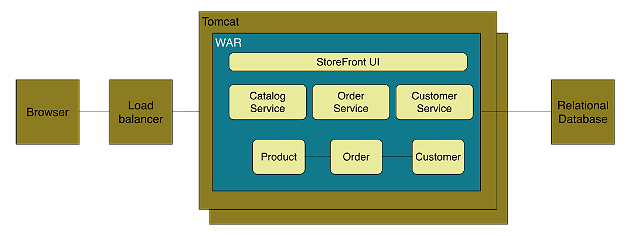
\includegraphics[width=0.7\textwidth]{figures/context-monolith-example}
\caption{Monolith Example from \cite{Richardson:2014aa}}
\label{fig:context/monolith-example}
\end{center}
\end{figure}

\subsection{Types of Monolith Architecture Style}\label{subsection:context/monolith-types}
According to \cite{Annett:2014aa}, a monolith can be of several types depending upon the viewpoint, as shown below:
\begin{enumerate}
\item Module Monolith: If all the code to realize an application share the same codebase and need to be compiled together to create a single artifact for the whole application then the architecture is Module Monolith Architecture. An example is show in Figure \ref {fig:context/module-monolith-example}. The application on the left of the figure, has all the code in the same codebase in the form of packages and classes without clear definition of modules and get compiled to a single artifact. However, the application on the right is developed as a number of modular codebase, each has separate codebase and can be compiled to different artifact. The modules uses the produced artifacts which is different than the earlier case where the code referenced each other directly.
\begin{figure}[H]
\begin{center}
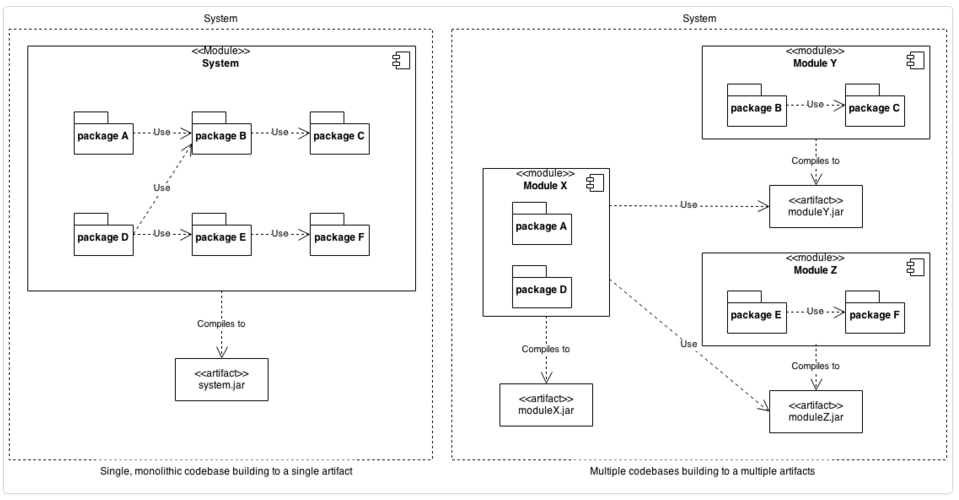
\includegraphics[width=0.8\textwidth]{figures/context-module-monolith}
\caption{Module Monolith Example from \cite{Annett:2014aa}}
\label{fig:context/module-monolith-example}
\end{center}
\end{figure}
\\
\item Allocation Monolith: An Allocation Monolith is created when all code is deployed to all the servers as a single version. This means that all the components running on the servers have the same versions at any time. The Figure \ref{fig:context/allocation-monolith-example} gives an example of allocation monolith. The system on the left have same version of artifact for all the components on all the servers. It does not make any differenct whether or not the system has single codebase and artifact. However, the system on the right as shown in the figure is realized with multiple version of the artifacts in different servers at any time.
\begin{figure}[H]
\begin{center}
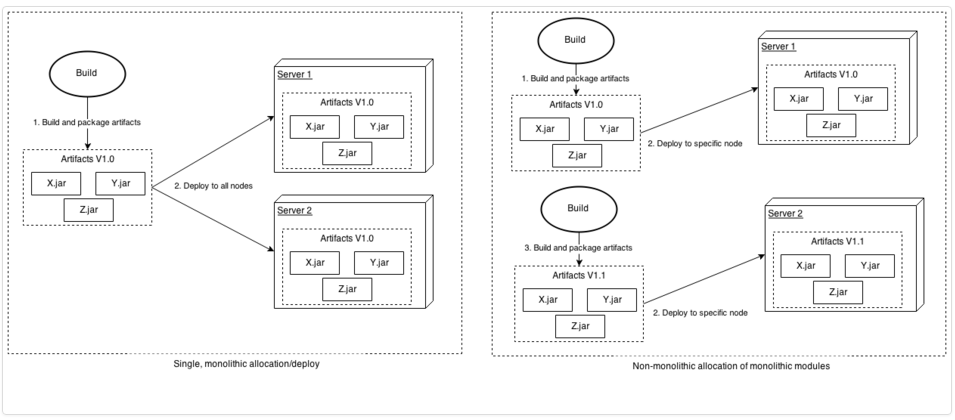
\includegraphics[width=0.8\textwidth]{figures/context-allocation-monolith}
\caption{Allocation Monolith Example from \cite{Annett:2014aa}}
\label{fig:context/allocation-monolith-example}
\end{center}
\end{figure}
\\
\item Runtime Monolith: In Runtime Monolith, the whole application is run under a single process. The left system in the Figure \ref{fig:context/runtime-monolith-example} shows an example of runtime monolith where a single server process is responsible for whole application. Whereas the system on the right has allocated multiple server process to run distinct set of component artifacts of the application.
\begin{figure}[H]
\begin{center}
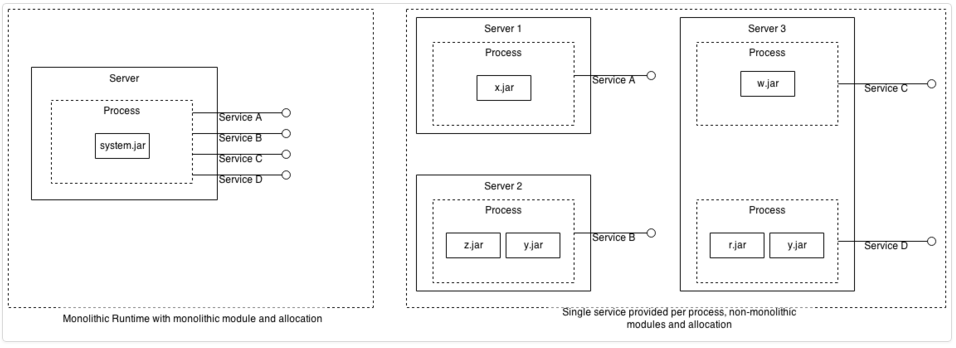
\includegraphics[width=0.8\textwidth]{figures/context-runtime-monolith}
\caption{Runtime Monolith Example from \cite{Annett:2014aa}}
\label{fig:context/runtime-monolith-example}
\end{center}
\end{figure}
\end{enumerate}

\\
\subsection{Advantages of Monolith Architecture Style}\label{subsection:context/monolith-advantages}
The Monolith architecture is appropriate for small application and has following benifits:\cite{Richardson:2014ab}\cite{Fowler:2014aa}\cite{Gupta:2015aa}\cite{Abram:2014aa}
\begin{itemize}[leftmargin=.5in]
\item It is easy to develop a monolith application since various development tools including \acrshort{IDE}s are created around the single application concept. Furthermore, it is also easy to test the application by creating appropriate environment on the developer's machine.
\item The deployment can be simply achieved by moving the single artifact for the application to an appropriate directory in the server.
\item The scaling can be clearly and easily done by replicating the application horizontally across multiple servers behind a load balancer as shown in Figure \ref{fig:context/monolith-example}
\item The different teams are working on the same codebase so sharing the functionality can be easier.
\end{itemize}
\\
\subsection{Disadvantages of Monolith Architecture Style}\label{subsection:context/monolith-disadvantages}
As the requirement grows with time, alongside application becomes huge and the size of team increases, then the monolith architecture faces many problems. The challenges of monolith architecture are as explained below:\cite{Namiot:2014aa}\cite{Newman:2015aa}\cite{Abram:2014aa}\cite{Richardson:2014aa}\cite{Richardson:2014ab}\cite{Gupta:2015aa}
\begin{itemize}[leftmargin=.5in]
\item Limited Agility: As the whole application has single codebase, even changing a small feature to release it in production takes time. Firstly, the small change can also trigger changes to other dependent code. In huge monolith application it is very difficult to manage modularity especially when all the team members are working on the same codebase. Secondly, to deploy a small change in production, the whole application has to be deployed. Thus continuous delivery gets slower. This will be more problematic when multiple changes have to be released on a daily basis. The slow pace and low frequency of release will highly affect agility.
\\
\item Decrease in Productivity: It is difficult to understand the application especially for a new developer because of the size of codebase. Although it also depends upon the structure of the codebase, it will still be difficult to grasp the significance of the code when there is no hard modular boundary. Additionally, a developer can be intimidated due to need to see the whole application at once from outwards to inwards direction. Secondly, the development environment can be slow to load the whole application and at the same time the deployment will also be slow. In overall, it will slow down the speed of understandability, execution and testing.
\\
\item Difficult Team Structure: The division of team as well as assigning tasks to the team can be tricky. Most common ways to partition teams in monolith are by technology and by geography. However, each one cannot be used in all the situations. In any case, the communication among the teams can be difficult and slow. Additionally, it is not easy to assign complete vertical ownership to a team for a particular feature from development to release. If something goes wrong in the deployment, there is always a confusion who should find the problem, either operations team or the last person to commit etc. The approprate team structure and ownership are very important for agility.
\\
\item Longterm Commitment to Technology stack: The technology to use is chosen before the development phase by analysing the requirements and the maturity of current technology at that time. All the teams in the architecture need to follow the same techonology stack throughout the lifecycle of application. However, if the requirement changes then there can be situation when the features can be best solved by different sets of technology. Additionally, not all the features in the application are same so cannot be treated accordingly and cannot be solved by same technology as well. Nevertheless, the technology advances rapidly. So, the solution thought right at the time of planning can be outdated and there can be a better solution available at present. In monolith application, it is very difficult to migrate to new technology stack and it can rather be a painfull process.
\\
\item Limited Scalability: The scaling of monolith application can be performed in either of two ways. The first way is to replicate the application along many servers and dividing the incoming request using a load balancer in front of the servers. Another approach is using identical copies of the application in multiple servers as in previous case but partitioning the database access instead of user request. Both of these scaling approaches improves the capacity and availability of the application. However, the individual requirement regarding scaling for each component can be different but cannot be fulfilled with this approach. Also, the complexity of the monolith application remains the same because we are replicating the whole application. Additionally, if there is a problem in a component the same problem can affect all the servers running the copies of the application, this does not improve resilency.\cite{MacVittie:2014aa}\cite{Namiot:2014aa}
\end{itemize}
\\

\section{Microservice Architecture Style}\label{section:context/microservices_architecture_style}
With monolith, it is easy to start development. But as the system gets bigger and complicated along time, it becomes very difficult to be agile and productive. The disadvantages listed in Section \ref{subsection:context/monolith-disadvantages} outweighs its advantages as the system gets old. The various qualities such as scalability, agility need to be maintained for the whole lifetime of the application and it becomes complicated by the fact that the system needs to be updated side by side because the requirements always keeps coming. In order to tackle these disadvantages, microservices architecture style is followed.\\
Microservices architecture uses the approach of decomposing an application into smaller autonomous components. The following Section \ref{section:context/microservices_architecture_style/decompostion_of_an_application} provides details of various decomposition techniques.

\subsection{Decomposition of an Application}\label{section:context/microservices_architecture_style/decompostion_of_an_application}
There are various ways to decompose an application. This section discuss two different ways of breaking down an application.

\subsubsection{Scale Cube}\label{section:context/microservices_architecture_style/decompostion_of_an_application/scale_cube}
The Section \ref{subsection:context/monolith-disadvantages} specified various disadvantages related to monolith architecture style. The book \cite{Fisher:2015aa} provides a way to solve most of the discussed problems related to agility, scalability, productivity etc. It provides three dimensions of scalability as shown in figure \ref{fig:context/scale-cube} which can be applied alone or simultaneously depending upon the situation and desired goals.

\begin{figure}[H]
\begin{center}
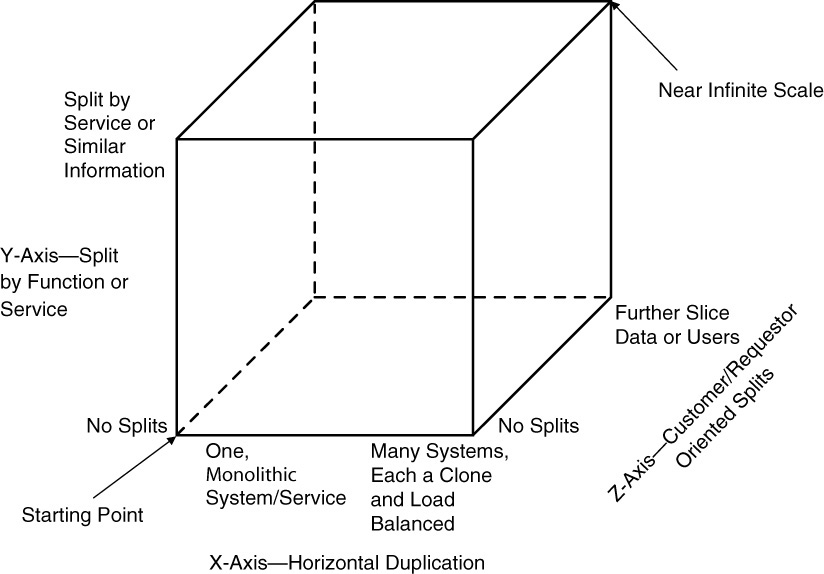
\includegraphics[width=0.5\textwidth]{figures/context-scale-cube}
\caption{Scale Cube from \cite{Fisher:2015aa}}}
\label{fig:context/scale-cube}
\end{center}
\end{figure}

\\
The scaling along each dimensions are described below. \cite{Fisher:2015aa}\cite{MacVittie:2014aa}\cite{Richardson:2014aa}
\begin{enumerate}
\item X-axis Scaling: It is achieved by cloning the application and data along multiple servers. A pool of requests are applied into a load balancer and the requests are deligated to any of the servers. Each of the server has the full capability of the application and full access to all the data required so in this respect it does not make any difference which server fulfills the request. Rather, it is about how many requests are fulfilled at any time. It is easy to scale along X-axis as the number of requests increases. The solution is as simple as to add additional clones. However, with this type of scaling, it does not scale with the increase in data. Moreover, it also does not scale when there are large variation in the frequency of any type of requests or there are dominant requests types because all the requests are handled in an unbiased way and allocated to servers in the same way.
\\
\item Z-axis Scaling: The scaling is obtained by spliting the request based on certain criteria or information regarding the requestor or customer affected by the request. It is different than X-axis scaling in the way that the servers are responsible for different kinds of requests. Normally, the servers have same copy of the application but some can have additional functionalies depending upon the requests expected. The Z-axis scaling helps in fault isolation and transaction scalability. Using this scaling, certain group of customers can be provided added functionality or a new functionality can be tested to a small group and thus minimizing the risk.
\\
\item Y-axis Scaling: The scaling along this dimension means the spliting of the application responsibility. The separation can be done either by data, by the actions performed on the data or by combination of both. The respective ways can be referred to as resoure-oriented or service-oriented splits. While the x-axis or z-axis split were rather duplication of work along servers, y-axis is more about specialization of work along servers. The major advantage of this scaling is that each request is scaled and handled differently according to its necessity. As the logic along with the data to be worked on are separated, developers can focus and work on small section at a time. This will increase productivity as well as agility. Additionally, a fault on a component is isolated and can be handled gracefully without affecting rest of the application. However, scaling along Y-axis can be costly compared to scaling along other dimensions.
\end{enumerate}
\subsubsection{Shared Libraries}\label{section:context/microservices_architecture_style/decompostion_of_an_application/shared_libraries}
Libraries is a standard way of sharing functionalities among various services and teams. The capability is provided by the feature of programming language. However there are various downsides to this approach. Firstly, it does not provide technology heterogeneity. Next, unless the library is dynamically linked, independent scaling, deployment and maintainance cannot be achieved. So, in other cases, any small change in the library leads to redeployment of whole system. Sharing code is a form of coupling which should be avoided.

Decomposing an application in terms of composition of individual features where each feature can be scaled and deployed independently, gives various advantages along agility, performance and team organization as well. Thus, microservices uses the decomposition technique presented by scale cube. A detail advantages of microservices are discussed further in Section \ref{section:challanges_of_microservices_architecture/introduction/challenges}.
\subsection{Definitions}\label{section:context/microservices_architecture_style/definitions}
There are several definitions given by several pioneers and early adapters of the style.
\\
\begin{shaded}Definition 1: \cite{Richardson:2014ac} \end{shaded}
"It is the way to functionally decompose an application into a set of collaborating services, each with a set of narrow, related functions, developed and deployed independently, with its own database."

\\
\begin{shaded}Definition 2: \cite{Wootton:2014aa}\end{shaded}
"It is a style of software architecture that involves delivering systems as a set of very small, granular, independent collaborating services."


\\
\begin{shaded}Definition 3: \cite{Cockcroft:2015aa}\end{shaded}
"Microservice is a loosely coupled Service-Oriented Architecture with bounded contexts."


\\
\begin{shaded}Definition 4: \cite{Fowler:2014aa}\cite{Radchenko:2015aa}\end{shaded}
"Microservices are Service-Oriented Architecture done right."


\\
\begin{shaded}Definition 5: \cite{Fowler:2014aa}\end{shaded}
"Microservice architecture style is an approach to developing a single application as a suite of small services, each running in its own process and communicating with lightweight mechanisms, often an HTTP resource API. These services are built around business capabilities and independently deployable by fully automated deployment machinery. There is a bare minimum of centralized management of these services, which may be written in different programming languages and use different data storage technologies."
\\
As other architectural styles, microservices presents its approach by increasing cohesion and decreasing coupling. Besides that, it breaks down system along business domains following single responsibility principle into granular and autonomous services running on separate processes. Additionally, the architecture focus on the collaboration of these services using light weight mechanisms.

\section{Motivation}\label{section:context/motivation}
The various definitions presented in section highlights different key terms such as:
\begin{enumerate}
\item collaborating services
\item developed and deployed independently
\item build around business capabilities
\item small, granular services
\end{enumerate}
These concepts are very important to be understood in order to approach microservices correctly and effectively. The first two terms relate to runtime operational qualities of microservices whereas the next two address modeling qualities. With that consideration, it indicates that the definitions provided are complete which focus on both aspects of any software applications. \\
However, if attempt is made to have clear indepth understanding of each of the key terms then various questions can be raised without appropriate answers. The various questions (shown in column 'Questions') related to modeling and operations (shown in column 'Type') are listed in the Table \ref{tab:context/microservices_architecture_style/various_questions_related_to_microservices}.
\begin{table}[H]
  \centering
  \begin{adjustbox}{max width=\textwidth}
  \begin{tabular}{*{14}{|c}|}%%{|c|c|}
  \hline
  \# & Questions & Type\\
  \hline
  \hline
   1 & How small should be size of microservices? &  Modeling  \\ \hline
   2 & How does the collaboration among services happen? & Operation  \\ \hline
   3 & How to deploy and maintain independently when there are dependencies among services?& Operation   \\ \hline
   4 & How to map microservices from business capabilities? & Modeling\\ \hline
   5 & What are the challenges need to be tackled and how to? & Operation\\ \hline \hline
   \end{tabular}
\end{adjustbox}
  \caption{Various Questions related to Microservices}
  \label{tab:context/microservices_architecture_style/various_questions_related_to_microservices}
\end{table}
Without clear answer to these questions, it is difficult to say that the definitions presented in Section \ref{section:context/microservices_architecture_style/definitions} are complete and enough to follow the microservices architecture. The process of creating microservices is not clearly documented. There is no enough research papers defining a thorough process of modeling and operating microservices. Additionally, a lot of industries such as amazon, netflix etc are following this architecture but it is not clear about the process they are using to define and implement microservices. The purpose of the research is to have a clear understanding about the process of designing microservices by focusing on following questions.
\begin{shaded}
\textbf{Research Questions}\label{list:introduction/research_questions}
\end{shaded}
\begin{enumerate}
\item How are boundary and size of microservices defined?
\item How business capabilities are mapped to define microservices?
\item What are the best practices to tackle challenges introduced by microservices?
    \begin{enumerate}
    \item How does the collaboration among services happen?
    \item How to deploy and maintain independently when there are dependencies among services?
    \item How to monitor microservices?
    \end{enumerate}
\end{enumerate}
\section{Research Approach}\label{section:context/approach}
A research is an iterative procedure with a goal of collecting as many relevant documents as possible so that the research questions could be answered rationally. So, it becomes very important to follow a consistent research procedure. For the current research, the approach is chosen by refering to \cite{np:2007aa}. It consists of two major phases.
\begin{enumerate}
\item {Data Collection Phase}
\item {Data Synthesis Phase}
\end{enumerate}
The following sections explains each phase in detail.
\subsection{Data Collection Phase}\label{section:context/approach/data_collection_phase}
In this phase, papers related to the reseach questions are collected. The Figure \ref{fig:context/data_collection_phase} shows basic steps in this phase.
\begin{figure}[H]
\begin{center}
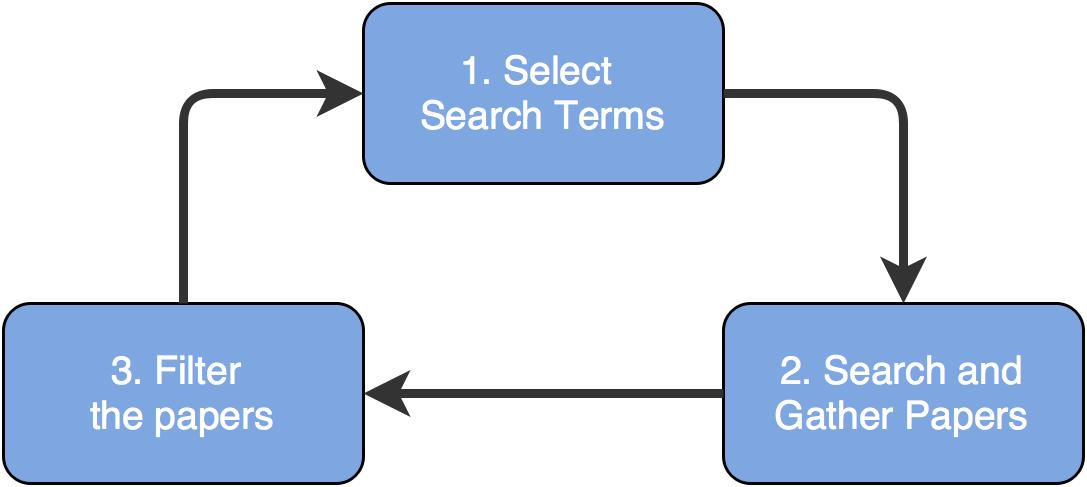
\includegraphics[width=0.8\textwidth]{figures/introduction_data_collection_phase}
\caption{Data Collection Phase}
\label{fig:context/data_collection_phase}
\end{center}
\end{figure}

\begin{enumerate}
\item \textbf{Select Search Terms}\\
At first, various search terms which defines the research topics and questions well, are selected using following strategies.
\begin{enumerate}
\item keywords from research questions and various definitions
\item synonyms of keywords
\item accepted and popular terms from academics and industries
\item references discovered from selected papers
\end{enumerate}
A consise list of initial keywords which are selected from various definitions of microservices are listed in Table \ref{tab:context/microservices_architecture_style/keywords_extracted_from_various_definitions_of_microservice}.
\item \textbf{Search and Gather Papers}\\
The search terms selected in previous step are utilized to discover various papers. In order to achieve that, the search terms are used against various resources listed below.
\begin{enumerate}
\item google scholar
\item IEEExplore
\item ACM Digital Library
\item Researchgate
\item Books
\item Technical Articles
\end{enumerate}
\item \textbf{Filter the Papers}
Finally, the various papers collected from various resources are filtered first to check if the papers have profound base to back up their result. Using only authentic papers is important to provide rational base to current research. The various criteria used to filter the papers are listed below.
\begin{enumerate}
\item Is the paper relevant to answer the research question?
\item Does the paper have good base in terms of sources and provide references of the past studies? 
\item Are there any case studies or examples provided to verify result of the reseach?
\end{enumerate}
\end{enumerate}

\subsection{Data Synthesis Phase}\label{section:context/approach/data_synthesis_phase}
The next phase is to gather data from the selected papers to create meaningful output and provide direction to the research. The Figure \ref{fig:context/data_synthesis_phase} shows various steps within this phase.
\begin{figure}[H]
\begin{center}
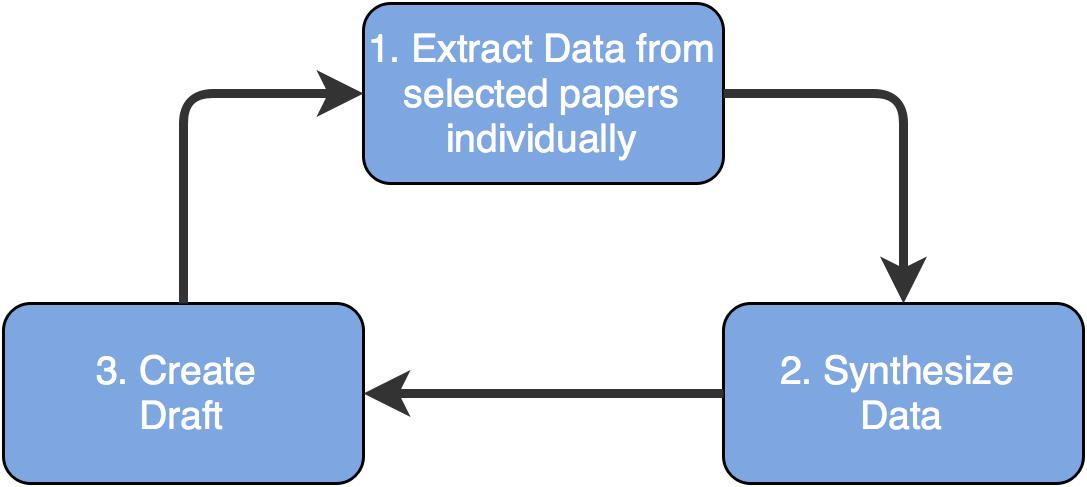
\includegraphics[width=0.8\textwidth]{figures/introduction_data_synthesis_phase}
\caption{Data Synthesis Phase}
\label{fig:context/data_synthesis_phase}
\end{center}
\end{figure}

\begin{enumerate}
\item \textbf{Extract Data from selected papers individually}\\
Firstly, each papers are scanned and important data relevant to research are collected.
\item \textbf{Synthesize Data}\\
The data collected from each paper are revised and compared for their similarities in concepts as well as differences in opinion. These individual contents from all papers are then synthesized.
\item \textbf{Create Draft}\\
Finally, draft for the observations are created for future reference which will be used later for creating final report.
\end{enumerate}


\section{Research Strategy}\label{section:context/research_strategy}
The Section \ref{section:context/approach} emphasize the importance of having consistent research procedure. Additionally, it is important to define a good strategy for achieving goals of the research. A good strategy is to narrow down the areas for conducting research. In this section, a list of areas will be identified.\\
The various definitions in Section \ref{section:context/microservices_architecture_style/definitions} show that the authors have their own interpretation of microservices but at the same time agree upon some basic concepts. Nevertheless, each definition can be used to understand different aspect of the microservices. A distinct set of keywords can be identified from these definitions which represents different aspects. The Table \ref{tab:context/microservices_architecture_style/keywords_extracted_from_various_definitions_of_microservice} shows various keywords to focus. Additionally, there are other columns in the table which represents various aspects of microservices architecture. These columns are checked or unchecked to represent the relevancy of each keyword. 

\begin{table}[H]
  \centering
  \begin{adjustbox}{max width=\textwidth}
  \begin{tabular}{*{14}{|c}|}%%{|c|c|c|c|c|c|}
  \hline
  \# & keywords & size & Quality of good microservice & communication & process to model microservices\\
  \hline
  \hline
   1 & Collaborating Services                                       &   &   & \checkmark &  \\ \hline
   2 & Communicating with lightweight mechanism like http           &   &   & \checkmark &  \\ \hline
   3 & Loosely coupled, related functions                           &   & \checkmark  & \checkmark &   \\ \hline
   4 & Developed and deployed independently       &  &   &  & \checkmark \\ \hline
   5 & Own database                                 &  & \checkmark &  & \checkmark \\ \hline
   6 & Different database technologies         &  &  &  & \checkmark \\ \hline
   7 & Service Oriented Architecture  & & \checkmark &  & \checkmark \\ \hline
   8 & Bounded Context  & \checkmark & \checkmark &  & \checkmark \\ \hline
   9 & Build around Business Capabilities  & \checkmark & \checkmark &  &\checkmark \\ \hline
   10 & Different Programming Languages & &  & & \checkmark \\ \hline
   \hline
   \end{tabular}
\end{adjustbox}
  \caption{Keywords extracted from various definitions of Microservice}
  \label{tab:context/microservices_architecture_style/keywords_extracted_from_various_definitions_of_microservice}
\end{table}
Finally, answering various questions around these keywords can be the \textbf{first approach} to understand the topics shown in columns such as size, quality of microservices etc.
\\
The \textbf{next approach} to look around the architecture process is to understand its various drivers. According to \cite{Brown:2015aa}, the important drivers which clarify the architecture are: 
\label{list:introduction/drivers}
\begin{enumerate}
\item \textbf{Quality Attributes}\\
The non-functional requirements have high impact on the resulting architecture. It is important to consider various quality attributes to define the process of architecture.
\item \textbf{Constraints}\\
There are always limitations or disadvantages faced by any architecture however the better knowledge is useful in the process of explaining the architecture with satisfaction.
\item \textbf{Principles}\\
The various principles provides a consistent approaches to tackle various limitations. They are the keys to define guidelines.
\end{enumerate}
So, in order to define the process of modeling microservices, the key aspects related to \textbf{quality attributes}, \textbf{constraints} and \textbf{principles} will be studied thoroughly.
\\
\\
Considering both the Table \ref{tab:context/microservices_architecture_style/keywords_extracted_from_various_definitions_of_microservice} and List \ref{list:introduction/drivers}, the approach to be used to define the guidelines will be to first look deep into various quality attributes influencing microservices architecture. Then, the process of identifying or modeling individual microservices from problem domain will be defined. At first, the research is performed based on various research papers. Then, the approach used by industry adopting microservices architecture will be studied in order to answer the research questions. The study will be performed on SAP Hybris.
Finally, the various constraints or challenges which affects microservices will be identified. 
The results of previous research will be mapped into a form of various principles and these principles will ultimately provide sufficient ground to create guidelines for microservices architecture.

\section{Problem Statement}\label{section:context/problem_statement}
Considering the case that the size of microservice is an important concept and is discussed a lot, but no concrete answer regarding this topic exists. Moreover, the idea of size has a lot of interpretations and no definite answer regarding how small a microservice should be. So, the first step should be to understand the concept of granularity in the context of microservices. Additionally, it would be great if some answers regarding the appropriate size of microservices could be found.

% later\chapter{Literature Review}\label{chapter:literature_review}
\section{Software Architecture}\label{section:software_architecture}


\begin{definition}[Software architecture \cite{bass_sa}]



%later\chapter{System Design}
\label{chapter:system_design}
%later\chapter{Results}
\label{chapter:results}

%later\chapter{Discussions}\label{chapter:discussions}
%later\chapter{Conclusion}\label{chapter:conclusion}
% What you learned
% What went well, bad, surprises, insights
% How you'd do it differently?
The software architecture provides a set of guidelines to decompose a system into subsystems, components and modules. Additionally, it defines the interaction amongst its individual components. Defining an architecture is an important part in software development. So, there should be precise guidelines to implement the architecture.\\
One of the architectural approaches is monolithic architecture in which an application is deployed as a single artifact. With this architecture, a) development, b) deployment and c) scaling is simple as long as the application is small. However, as the application gets bigger and complex, the architecture faces various disadvantages including a) limited agility, b) decrease in productivity, c) longterm commitment to technology stack, d) limited scalability, etc. This is where, a different architectural approach called 'Microservices' comes into play. In this approach, a) an application is composed using different independent, autonomous components, b) each component fulfils a single functionality and  c) each component can be deployed as well as updated independently. However, there are various concepts related to the definitions of microservices such as collaboration, granularity, mapping of business capability, etc. which are not clearly documented. Moreover, there are no proper guidelines how to follow microservices architecture. This is the motivation of the current research. The objective of the research is to clarify various concepts related to the microservices and finally create a precise guidelines for implementing the microservices.\\
In order to achieve that, various definitions provided by different authors are taken as starting point. A list of keywords and areas are selected from them, which are further investigated during the research. Furthermore, various factors such as a) quality attributes, b) constraints and c) principles are considered as the building blocks of any architecture. So, these areas are also considered during the research to create guidelines.\\
Granularity of a microservice is considered as an important concept and is discussed a lot. Granularity is not a one dimensional entity but has three distinct dimensions which are a) functionality, b) data and c) business value. Increase in any of these dimension increases granularity. Also, it is important to consider the concept of 'Appropriate' granularity rather than 'Minimum' sized microservices. Appropriate granularity of any microservice is achieved by three basic concepts: \textbf{Single Responsibility Principle}, \textbf{Autonomy}, and \textbf{Infrastructure capability}.
\\
Adding to that, other quality attributes such as coupling, cohesion, autonomy, etc. are as important as granularity. For that purpose, a list of basic metrics are created to evaluate each quality attributes easily. The quality attributes are not mutually exclusive but related to eachother. The relationship among them is clarified so that it becomes easy to determine the appropriate tradeoffs when necessary.\\
Another important concept which is not clearly documented is the process of identification of microservices and mapping of business capability to microservices. Two different approaches are discussed which are \textbf{Using Use Cases Refactoring} and  \textbf{Using Domain Driven Design}.\\
Use Cases Refactoring utilizes use cases to breakdown a problem domain and refactor them based on various concepts such as similarity in functionality, similarity on entities they act, etc. A discrete set of rules for use cases refactoring are also present. On the other hand, domain driven design uses the concept of ubiquitous language and bounded context to break down a problem domain. A detailed step for each phase is also presented. Furthermore, a case study is broken down into microservices using each approach.\\
Use cases Refactoring is comparatively easier since architects and developers are more familiar with the concept. Domain Driven Design on the other hand, is a complex and iterative procedure. Furthermore, use cases Refactoring considers an entity as a single source of truth for all sub-domains in the entire system. Using this approach does not necessarily produce autonomous microservices but focus more on functionalities. However, the domain driven design using the concept of ubiquitous language and bounded context creates autonomous microservices with single responsibility.\\
After conducting research along various literature, another important part is determining the process followed in industry for which SAP Hybris is chosen. Firstly, various available documents are studied which suggested vision and principles as being the driving force for the process of implementing microservices. In order to understand indepth, interviews are conducted with various key personnels related to \acrshort{YaaS}. A major outcome of the interview is that, in addition to factors such as autonomy, infrastructure capability and Single Responsibility Principle, \textbf{Business Value} of the microservices plays significant role when a) identifying microservices  and b) defining the optimum granularity. Finally, the workflow followed during deployment of microservices in SAP Hybris is also studied in order to clarify the operational approach together with modeling process.\\
Understanding constraints is another important driver of architecture. The approach to handle various constraints can be helpful in defining guidelines. Microservices architecture has various advantages such as strong modularity, agility, independent deployment capability however also presents various challenges for maintaining these advantages. The challenges can be kept into three distinct groups: 
\textbf{Distributed System Complexity}
\textbf{Integration}, and
\textbf{Operational Complexity}.\\
Different challenges along each group are discussed. Additionally, the various techniques which can be used to tackle each  are listed based on the literature. Finally, the techniques used in SAP Hybris to handle each challenge are also mentioned.\\
With all the studies performed, the process of microservices architecture can be disected along two phases:
\textbf{Modeling Phase} and 
\textbf{Operation Phase}.\\
During the modeling phase, problem domain is studied and various internal quality attributes along with business value as well as infrastructure capability are considered. Whereas during operational phase, various challenges are tackled. The effectiveness of modeling phase is visible across various external quality attributes in operation phase. Again, the principles are major driving factor for creating architectural guidelines. The principles along both modeling and operation phase are listed based on the previous findings of the research. Finally, for each principles, a set of guidelines are presented. The guidelines are one of the major outcomes of the research.

%later\chapter{Future Directions}\label{chapter:future_directions}
The current thesis research is conducted on the basis of various academic as well as industrial researches. It would be interesting if the current research could create opportunities for new researches.\\
The Table \ref {tab:quality_of_service/quality_attributes/basic_quality_metrics} listed some basic metrices which can be used to evaluate the quality of microservices. The very first thing which can be done is to find the threshold range that can classify good and bad microservices. A certain number of microservices can be taken as sample from which microservices with high scalability, reusability or other external quality attributes can be filtered out from non performing microservices with low scalability and reusability. Then basic metrices tables can be filled along with their corresponding values for each microservice. These tables can used to find threshold values. The threshold values can be verified further by using them while creating new microservice and checking if their external quality attributes meet the expectations.\\
Another direction of the research can be finding the priority sequence of quality attributes for microservices. From literature, the quality attributes to focus are coupling, cohesion and autonomy. During the interview conducted with SAP Hybris, the quality attributes such as scalability and reusability were given priority when mapping functionalities to microservices. It can be valuable to research further in literature as well as in other industries regarding the priority of quality attributes they choose to identify microservices.\\
Furthermore, the basic metrices table can be leveraged to create a graphical tool which representes various microservices as nodes and connections between them as lines between nodes. It would be benefical if various basic metrices can be evaluated only with \acrshort{API} definitions automatically. Then, the graphical tool can be used to show the various quality attributes using the basic metrices. Depending upon the expected quality, the graphical tool can be used to change the definitiona or \acrshort{API} definition can be changed directly. This can be a great interactive tool for optimizing quality of microservices at design time.\\
Nevertheless, the report can always be used as a base to conduct research on other similar industries as SAP Hybris. It can be interesting to view the result obtained from the study at various different industries.
Given the situation that there are very few literature research done in this area and most of the industries which are using microservices have not openly communicated the whole lifecycle process of microservices, this document can be a very good resource for any company to implement microservices architecture. Additionally, the document can also be a good source for further researches in this area.

%later\chapter{Appendices}\label{chapter:appendices}

\section{CAP Theorem}\label{section:appendices/CAP_theorem}
CAP Theorem was published by scientist Eric Brewer and also called as Brewer's Theorem. There are three major requirements for deploying an application in a distributed environment.
\begin{enumerate}
\item \textbf{Consistency}\\
A functionality of a service is accomplished as a whole or not at all. All the nodes accessing any data see the same version at any given time.
\item \textbf{Availability}\\
The functionalities provided by a service are available and working.
\item \textbf{Partition Tolerance}\\
The partitions which occurs due to problems in the network does not affect the operations of the system unless the whole network fails.
\end{enumerate}
According to the theorem, as the system scales across a number of nodes and the volume of requests increase, it becomes difficult to achieve all the three qualities but to compromise any one of them. \cite{Julian:2009aa}
Network partitions cannot be avoided completely due to the very nature of distributed system and so is the quality of partition tolerance has to be maintained. The choice is the trade off between availability and consistency. It is completely dependent upon business requirement which one to choose. \cite{Peter-Bailis:2013aa}
\section{Eventual Consistency}\label{section:appendices/eventual_consistency}
It is a weaker form of consistency which guarantees all read to a data item return the same value eventually, if no additional updates are performend to the same data item. For any update, only the nodes which are viable and reachable at the moment are updated and the remaining nodes are updated when they are back. \cite{Peter-Bailis:2013aa}
\section{Command Query Responsibility Segregation(CQRS)}\label{section:appendices/CQRS}
In this pattern as shown in the figure \ref{fig:appendices/cqrs}, the conceptual model is divided into two separate models, each one for update and read. It refers to creating different object model handled by different logical processes. The database can be shared, where it acts as integration point but can have different database as well.

\begin{figure}[H]
\begin{center}
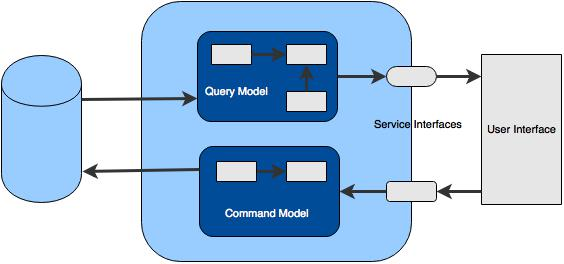
\includegraphics[width=0.8\textwidth]{figures/Appendices_one_cqrs}
\caption{CQRS [\cite{Fowler:2011ab}]}
\label{fig:appendices/cqrs}
\end{center}
\end{figure}

\section{Single Responsibility Principle}\label{section:appendices/single_responsibility_principle}
Responsibility is inferred as a reason to change. According to the principle, a service should have a single reson to change. In order to achieve that, a service should perform functionalities which change for the same reason. \cite{Martin:2009aa} \cite{Stine:2014aa}

\appendix{}

\glsaddall{} % add all defined terms to glossary, even if not referenced in text
%\printglossaries{}
\printglossary[type=\acronymtype]

\microtypesetup{protrusion=false}
\listoffigures{}
%later\listoftables{}
\microtypesetup{protrusion=true}
\printbibliography{}

\end{document}
